\documentclass[a4paper]{book}
\usepackage{a4wide}
\usepackage{makeidx}
\usepackage{graphicx}
\usepackage{multicol}
\usepackage{float}
\usepackage{listings}
\usepackage{color}
\usepackage{textcomp}
\usepackage{alltt}
\usepackage{times}
\usepackage{ifpdf}
\ifpdf
\usepackage[pdftex,
            pagebackref=true,
            colorlinks=true,
            linkcolor=blue,
            unicode
           ]{hyperref}
\else
\usepackage[ps2pdf,
            pagebackref=true,
            colorlinks=true,
            linkcolor=blue,
            unicode
           ]{hyperref}
\usepackage{pspicture}
\fi
\usepackage[utf8]{inputenc}
\usepackage{polski}
\usepackage[T1]{fontenc}

\usepackage{doxygen}
\lstset{language=C++,inputencoding=utf8,basicstyle=\footnotesize,breaklines=true,breakatwhitespace=true,tabsize=8,numbers=left }
\makeindex
\setcounter{tocdepth}{3}
\renewcommand{\footrulewidth}{0.4pt}
\begin{document}
\hypersetup{pageanchor=false}
\begin{titlepage}
\vspace*{7cm}
\begin{center}
{\Large Bazinga Camera Driver \\[1ex]\large 0.1 }\\
\vspace*{1cm}
{\large Wygenerowano przez Doxygen 1.6.3}\\
\vspace*{0.5cm}
{\small Mon Mar 15 22:10:02 2010}\\
\end{center}
\end{titlepage}
\clearemptydoublepage
\pagenumbering{roman}
\tableofcontents
\clearemptydoublepage
\pagenumbering{arabic}
\hypersetup{pageanchor=true}
\chapter{Indeks klas}
\section{Hierarchia klas}
Ta lista dziedziczenia posortowana jest z grubsza, choć nie całkowicie, alfabetycznie:\begin{DoxyCompactList}
\item \contentsline{section}{CameraNotConnectedBlocker}{\pageref{class_camera_not_connected_blocker}}{}
\item \contentsline{section}{FrameRetreiver}{\pageref{class_frame_retreiver}}{}
\begin{DoxyCompactList}
\item \contentsline{section}{ConfigDialog}{\pageref{class_config_dialog}}{}
\item \contentsline{section}{Faces}{\pageref{class_faces}}{}
\item \contentsline{section}{Points2}{\pageref{class_points2}}{}
\item \contentsline{section}{Quadrangles}{\pageref{class_quadrangles}}{}
\end{DoxyCompactList}
\item \contentsline{section}{ImageDisplayer}{\pageref{class_image_displayer}}{}
\item \contentsline{section}{VideoInput}{\pageref{class_video_input}}{}
\end{DoxyCompactList}

\chapter{Indeks klas}
\section{Lista klas}
Tutaj znajdują się klasy, struktury, unie i interfejsy wraz z ich krótkimi opisami:\begin{DoxyCompactList}
\item\contentsline{section}{\hyperlink{class_idiot_window}{IdiotWindow} (Klasa wyświetlająca okno programu )}{\pageref{class_idiot_window}}{}
\item\contentsline{section}{\hyperlink{class_image_widget}{ImageWidget} (Wyświetla obiekty od klientów w różnych kolorach )}{\pageref{class_image_widget}}{}
\end{DoxyCompactList}

\chapter{Dokumentacja klas}
\hypertarget{class_camera_not_connected_blocker}{
\section{Dokumentacja klasy CameraNotConnectedBlocker}
\label{class_camera_not_connected_blocker}\index{CameraNotConnectedBlocker@{CameraNotConnectedBlocker}}
}
\subsection*{Metody publiczne}
\begin{DoxyCompactItemize}
\item 
\hypertarget{class_camera_not_connected_blocker_a36847155966f5fded3d9d5ae9a348be7}{
{\bfseries CameraNotConnectedBlocker} (\hyperlink{class_config_dialog}{ConfigDialog} $\ast$cdialog)}
\label{class_camera_not_connected_blocker_a36847155966f5fded3d9d5ae9a348be7}

\item 
\hypertarget{class_camera_not_connected_blocker_a6a2b84c9469178c7bdc3a40279ba17eb}{
bool {\bfseries canConnect} ()}
\label{class_camera_not_connected_blocker_a6a2b84c9469178c7bdc3a40279ba17eb}

\item 
\hypertarget{class_camera_not_connected_blocker_adc130d65f47c9e7d2a07d032c3f62ba5}{
QString {\bfseries toString} ()}
\label{class_camera_not_connected_blocker_adc130d65f47c9e7d2a07d032c3f62ba5}

\end{DoxyCompactItemize}


Dokumentacja dla tej klasy została wygenerowana z plików:\begin{DoxyCompactItemize}
\item 
cameranotconnectedblocker.h\item 
cameranotconnectedblocker.cpp\end{DoxyCompactItemize}

\hypertarget{class_config_dialog}{
\section{Dokumentacja klasy ConfigDialog}
\label{class_config_dialog}\index{ConfigDialog@{ConfigDialog}}
}
Klasa wyświetlająca okno konfiguracyjne.  


{\tt \#include $<$configdialog.h$>$}

Diagram dziedziczenia dla ConfigDialog:\begin{figure}[H]
\begin{center}
\leavevmode
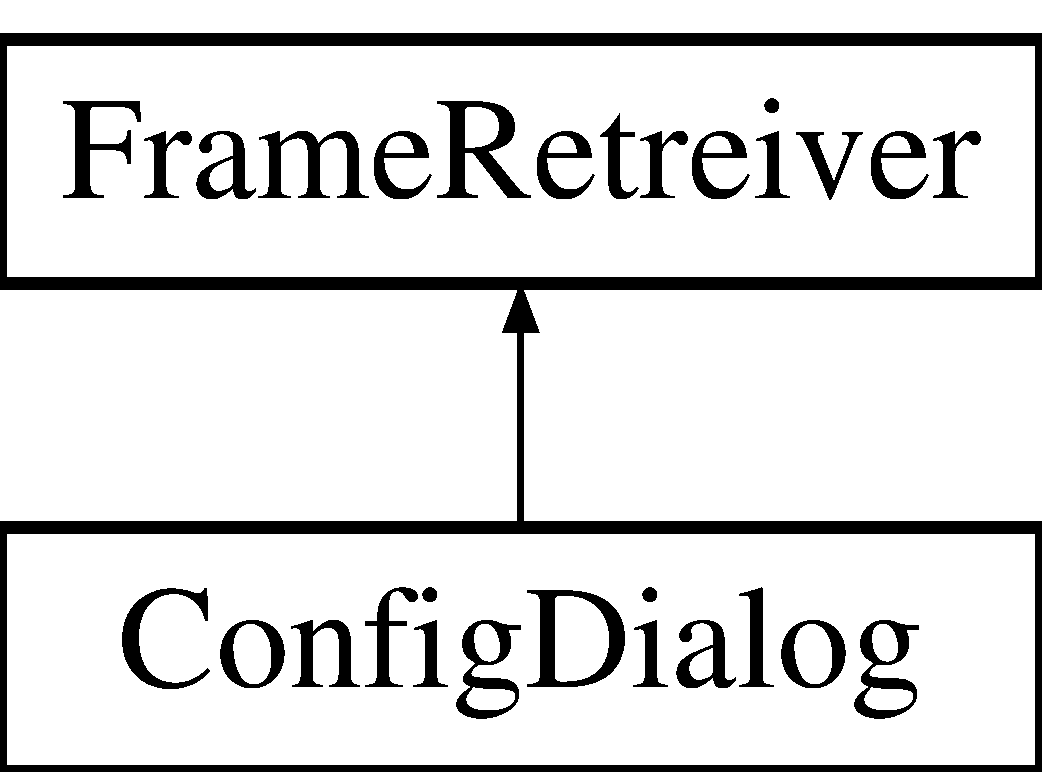
\includegraphics[height=2cm]{class_config_dialog}
\end{center}
\end{figure}
\subsection*{Sloty publiczne}
\begin{CompactItemize}
\item 
\hypertarget{class_config_dialog_21d23a581bbbf582c4a25d7d7204e764}{
void \hyperlink{class_config_dialog_21d23a581bbbf582c4a25d7d7204e764}{connectCamera} ()}
\label{class_config_dialog_21d23a581bbbf582c4a25d7d7204e764}

\begin{CompactList}\small\item\em Podłącza kamerę. \item\end{CompactList}\item 
\hypertarget{class_config_dialog_4e9e42e4decdb4f6895f4b47d51b550e}{
void \hyperlink{class_config_dialog_4e9e42e4decdb4f6895f4b47d51b550e}{disconnectCamera} ()}
\label{class_config_dialog_4e9e42e4decdb4f6895f4b47d51b550e}

\begin{CompactList}\small\item\em Rozłącza kamerę. \item\end{CompactList}\item 
void \hyperlink{class_config_dialog_5611fa4c9de2827139161cd75a7f4be6}{serverConnected} (quint32 sessid)
\begin{CompactList}\small\item\em Wywołaj, żeby poinformować okno o nawiązaniu połączenia. \item\end{CompactList}\item 
void \hyperlink{class_config_dialog_7782fa76c40b70438677baff0c2622f2}{serverDisconnected} ()
\begin{CompactList}\small\item\em Wywołaj, żeby poinformować okno o rozwiązaniu połączenia. \item\end{CompactList}\item 
void \hyperlink{class_config_dialog_dfe6884aef5e1c04ce574c6c9a1a97d9}{saveSettings} ()
\begin{CompactList}\small\item\em Zapisz ustawienia. \item\end{CompactList}\item 
\hypertarget{class_config_dialog_06d4edc9ec519809ce9104b66b15dadf}{
void \hyperlink{class_config_dialog_06d4edc9ec519809ce9104b66b15dadf}{readSettings} ()}
\label{class_config_dialog_06d4edc9ec519809ce9104b66b15dadf}

\begin{CompactList}\small\item\em Odczytaj ustawienia. \item\end{CompactList}\item 
\hypertarget{class_config_dialog_99f28a7e313ccc20892503afdc3191b9}{
void \hyperlink{class_config_dialog_99f28a7e313ccc20892503afdc3191b9}{catchException} (BConnectionException $\ast$e)}
\label{class_config_dialog_99f28a7e313ccc20892503afdc3191b9}

\begin{CompactList}\small\item\em Wyświetl komunikat z treścią wyjątku. \item\end{CompactList}\end{CompactItemize}
\subsection*{Metody publiczne}
\begin{CompactItemize}
\item 
\hyperlink{class_config_dialog_d16df8ed2e55bd5cc55e3ef9040b8b93}{ConfigDialog} (QWidget $\ast$parent=0)
\begin{CompactList}\small\item\em Konstruktor. \item\end{CompactList}\item 
\hyperlink{class_config_dialog_485badac4dffa04603f800bb9d396e1d}{$\sim$ConfigDialog} ()
\begin{CompactList}\small\item\em Destruktor. \item\end{CompactList}\end{CompactItemize}
\subsection*{Przyjaciele}
\begin{CompactItemize}
\item 
bool \hyperlink{class_config_dialog_3b0963bb150b18a9cbd3b46187f7ea26}{CameraNotConnectedBlocker::canConnect} ()
\end{CompactItemize}


\subsection{Opis szczegółowy}
Klasa wyświetlająca okno konfiguracyjne. 

\subsection{Dokumentacja konstruktora i destruktora}
\hypertarget{class_config_dialog_d16df8ed2e55bd5cc55e3ef9040b8b93}{
\index{ConfigDialog@{ConfigDialog}!ConfigDialog@{ConfigDialog}}
\index{ConfigDialog@{ConfigDialog}!ConfigDialog@{ConfigDialog}}
\subsubsection[{ConfigDialog}]{\setlength{\rightskip}{0pt plus 5cm}ConfigDialog::ConfigDialog (QWidget $\ast$ {\em parent} = {\tt 0})}}
\label{class_config_dialog_d16df8ed2e55bd5cc55e3ef9040b8b93}


Konstruktor. 

Ustawia connecty m/obiektami i włącza timer (2s) \hypertarget{class_config_dialog_485badac4dffa04603f800bb9d396e1d}{
\index{ConfigDialog@{ConfigDialog}!$\sim$ConfigDialog@{$\sim$ConfigDialog}}
\index{$\sim$ConfigDialog@{$\sim$ConfigDialog}!ConfigDialog@{ConfigDialog}}
\subsubsection[{$\sim$ConfigDialog}]{\setlength{\rightskip}{0pt plus 5cm}ConfigDialog::$\sim$ConfigDialog ()}}
\label{class_config_dialog_485badac4dffa04603f800bb9d396e1d}


Destruktor. 

Próbuje rozłączyć kamerę i połączenie. Zapisuje ustawienia 

\subsection{Dokumentacja funkcji składowych}
\hypertarget{class_config_dialog_dfe6884aef5e1c04ce574c6c9a1a97d9}{
\index{ConfigDialog@{ConfigDialog}!saveSettings@{saveSettings}}
\index{saveSettings@{saveSettings}!ConfigDialog@{ConfigDialog}}
\subsubsection[{saveSettings}]{\setlength{\rightskip}{0pt plus 5cm}void ConfigDialog::saveSettings ()\hspace{0.3cm}{\tt  \mbox{[}slot\mbox{]}}}}
\label{class_config_dialog_dfe6884aef5e1c04ce574c6c9a1a97d9}


Zapisz ustawienia. 

Zapisywane w destruktorze \hypertarget{class_config_dialog_5611fa4c9de2827139161cd75a7f4be6}{
\index{ConfigDialog@{ConfigDialog}!serverConnected@{serverConnected}}
\index{serverConnected@{serverConnected}!ConfigDialog@{ConfigDialog}}
\subsubsection[{serverConnected}]{\setlength{\rightskip}{0pt plus 5cm}void ConfigDialog::serverConnected (quint32 {\em sessid})\hspace{0.3cm}{\tt  \mbox{[}slot\mbox{]}}}}
\label{class_config_dialog_5611fa4c9de2827139161cd75a7f4be6}


Wywołaj, żeby poinformować okno o nawiązaniu połączenia. 

Już podłączone w konstruktorze \hypertarget{class_config_dialog_7782fa76c40b70438677baff0c2622f2}{
\index{ConfigDialog@{ConfigDialog}!serverDisconnected@{serverDisconnected}}
\index{serverDisconnected@{serverDisconnected}!ConfigDialog@{ConfigDialog}}
\subsubsection[{serverDisconnected}]{\setlength{\rightskip}{0pt plus 5cm}void ConfigDialog::serverDisconnected ()\hspace{0.3cm}{\tt  \mbox{[}slot\mbox{]}}}}
\label{class_config_dialog_7782fa76c40b70438677baff0c2622f2}


Wywołaj, żeby poinformować okno o rozwiązaniu połączenia. 

Już podłączone w konstruktorze 

\subsection{Dokumentacja przyjaciół i funkcji związanych}
\hypertarget{class_config_dialog_3b0963bb150b18a9cbd3b46187f7ea26}{
\index{ConfigDialog@{ConfigDialog}!CameraNotConnectedBlocker::canConnect@{CameraNotConnectedBlocker::canConnect}}
\index{CameraNotConnectedBlocker::canConnect@{CameraNotConnectedBlocker::canConnect}!ConfigDialog@{ConfigDialog}}
\subsubsection[{CameraNotConnectedBlocker::canConnect}]{\setlength{\rightskip}{0pt plus 5cm}bool CameraNotConnectedBlocker::canConnect ()\hspace{0.3cm}{\tt  \mbox{[}friend\mbox{]}}}}
\label{class_config_dialog_3b0963bb150b18a9cbd3b46187f7ea26}


Pozwala na dostęp do tego obiektu z metody sprawdzającej czy jest podłączona kamerka. 

Dokumentacja dla tej klasy została wygenerowana z plików:\begin{CompactItemize}
\item 
configdialog.h\item 
configdialog.cpp\end{CompactItemize}

\hypertarget{class_faces}{
\section{Dokumentacja klasy Faces}
\label{class_faces}\index{Faces@{Faces}}
}


Wykrywa twarze.  




{\ttfamily \#include $<$faces.h$>$}

Diagram dziedziczenia dla Faces\begin{figure}[H]
\begin{center}
\leavevmode
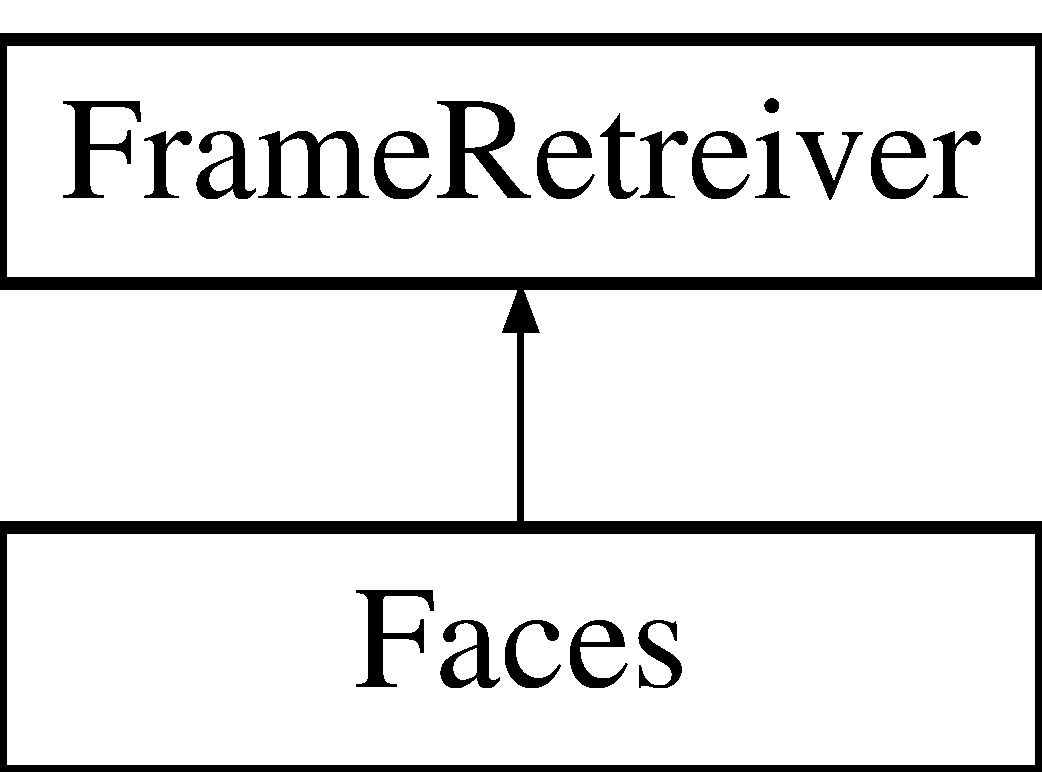
\includegraphics[height=2cm]{class_faces}
\end{center}
\end{figure}
\subsection*{Sygnały}
\begin{DoxyCompactItemize}
\item 
\hypertarget{class_faces_a92e42ecfad99d9e0766b569b562b86ba}{
void \hyperlink{class_faces_a92e42ecfad99d9e0766b569b562b86ba}{bobjects} (BObList $\ast$list)}
\label{class_faces_a92e42ecfad99d9e0766b569b562b86ba}

\begin{DoxyCompactList}\small\item\em emituje obiekty typu BOb \item\end{DoxyCompactList}\end{DoxyCompactItemize}
\subsection*{Metody publiczne}
\begin{DoxyCompactItemize}
\item 
\hypertarget{class_faces_a65ba31b6180506d6815f773365883a80}{
\hyperlink{class_faces_a65ba31b6180506d6815f773365883a80}{Faces} (\hyperlink{class_video_input}{VideoInput} $\ast$input)}
\label{class_faces_a65ba31b6180506d6815f773365883a80}

\begin{DoxyCompactList}\small\item\em Pobieraj z danego wejścia. \item\end{DoxyCompactList}\item 
void \hyperlink{class_faces_a7fd92e73e117b72898097551b964fd96}{retreiveFrame} (cv::Mat \&)
\begin{DoxyCompactList}\small\item\em Odbiera ramkę jako cv::Mat. \item\end{DoxyCompactList}\end{DoxyCompactItemize}


\subsection{Opis szczegółowy}
Wykrywa twarze. 

\subsection{Dokumentacja funkcji składowych}
\hypertarget{class_faces_a7fd92e73e117b72898097551b964fd96}{
\index{Faces@{Faces}!retreiveFrame@{retreiveFrame}}
\index{retreiveFrame@{retreiveFrame}!Faces@{Faces}}
\subsubsection[{retreiveFrame}]{\setlength{\rightskip}{0pt plus 5cm}void Faces::retreiveFrame (cv::Mat \& {\em mat})\hspace{0.3cm}{\ttfamily  \mbox{[}virtual\mbox{]}}}}
\label{class_faces_a7fd92e73e117b72898097551b964fd96}


Odbiera ramkę jako cv::Mat. 

do samodzielnej implementacji 

Reimplementowana z \hyperlink{class_frame_retreiver_a72912583af45c00d267f215a0d0b9bb1}{FrameRetreiver}.



Dokumentacja dla tej klasy została wygenerowana z plików:\begin{DoxyCompactItemize}
\item 
faces.h\item 
faces.cpp\item 
moc\_\-faces.cpp\end{DoxyCompactItemize}

\hypertarget{class_frame_retreiver}{
\section{Dokumentacja klasy FrameRetreiver}
\label{class_frame_retreiver}\index{FrameRetreiver@{FrameRetreiver}}
}
Klasa definiująca interfejs dla klas odbierających ramki obrazu.  


{\tt \#include $<$frameretreiver.h$>$}

Diagram dziedziczenia dla FrameRetreiver:\begin{figure}[H]
\begin{center}
\leavevmode
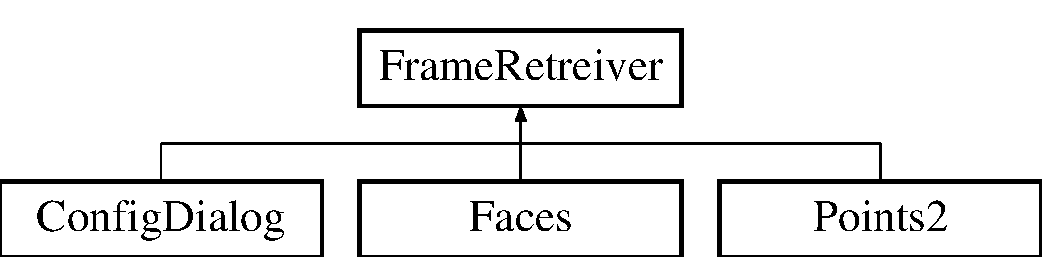
\includegraphics[height=2cm]{class_frame_retreiver}
\end{center}
\end{figure}
\subsection*{Metody publiczne}
\begin{CompactItemize}
\item 
\hyperlink{class_frame_retreiver_ec5e4a7cd0af2badc9b47fd3c936ac60}{FrameRetreiver} (\hyperlink{class_video_input}{VideoInput} $\ast$input)
\begin{CompactList}\small\item\em Konstruktor. \item\end{CompactList}\item 
void \hyperlink{class_frame_retreiver_8d7772f0a3d6373f5a54bf4fcc042ccc}{setInput} (\hyperlink{class_video_input}{VideoInput} $\ast$input)
\begin{CompactList}\small\item\em Ustawia wejście. \item\end{CompactList}\item 
\hypertarget{class_frame_retreiver_2345c5f4273008325ecfaf84f63d001c}{
virtual \hyperlink{class_frame_retreiver_2345c5f4273008325ecfaf84f63d001c}{$\sim$FrameRetreiver} ()}
\label{class_frame_retreiver_2345c5f4273008325ecfaf84f63d001c}

\begin{CompactList}\small\item\em Wypisuje się z obserwowanego wejścia. \item\end{CompactList}\item 
virtual void \hyperlink{class_frame_retreiver_061c97e43f3b73705903e49afad3e5bf}{retreiveFrame} (QImage \&)
\begin{CompactList}\small\item\em Odbiera ramkę jako QImage. \item\end{CompactList}\item 
virtual void \hyperlink{class_frame_retreiver_72912583af45c00d267f215a0d0b9bb1}{retreiveFrame} (cv::Mat \&)
\begin{CompactList}\small\item\em Odbiera ramkę jako cv::Mat. \item\end{CompactList}\end{CompactItemize}


\subsection{Opis szczegółowy}
Klasa definiująca interfejs dla klas odbierających ramki obrazu. 

Użytkownik implementuje jedną z dwóch metod \hyperlink{class_frame_retreiver_061c97e43f3b73705903e49afad3e5bf}{retreiveFrame()} 

\subsection{Dokumentacja konstruktora i destruktora}
\hypertarget{class_frame_retreiver_ec5e4a7cd0af2badc9b47fd3c936ac60}{
\index{FrameRetreiver@{FrameRetreiver}!FrameRetreiver@{FrameRetreiver}}
\index{FrameRetreiver@{FrameRetreiver}!FrameRetreiver@{FrameRetreiver}}
\subsubsection[{FrameRetreiver}]{\setlength{\rightskip}{0pt plus 5cm}FrameRetreiver::FrameRetreiver ({\bf VideoInput} $\ast$ {\em input})}}
\label{class_frame_retreiver_ec5e4a7cd0af2badc9b47fd3c936ac60}


Konstruktor. 

\begin{Desc}
\item[Parametry:]
\begin{description}
\item[{\em input}]powoduje, ze wszystkie ramki z inputu trafią też tu. \end{description}
\end{Desc}


\subsection{Dokumentacja funkcji składowych}
\hypertarget{class_frame_retreiver_72912583af45c00d267f215a0d0b9bb1}{
\index{FrameRetreiver@{FrameRetreiver}!retreiveFrame@{retreiveFrame}}
\index{retreiveFrame@{retreiveFrame}!FrameRetreiver@{FrameRetreiver}}
\subsubsection[{retreiveFrame}]{\setlength{\rightskip}{0pt plus 5cm}void FrameRetreiver::retreiveFrame (cv::Mat \& {\em mat})\hspace{0.3cm}{\tt  \mbox{[}virtual\mbox{]}}}}
\label{class_frame_retreiver_72912583af45c00d267f215a0d0b9bb1}


Odbiera ramkę jako cv::Mat. 

do samodzielnej implementacji 

Reimplementowana w \hyperlink{class_faces_7fd92e73e117b72898097551b964fd96}{Faces} i \hyperlink{class_points2_f46dd0cd21f73b3214d5f766349b8450}{Points2}.\hypertarget{class_frame_retreiver_061c97e43f3b73705903e49afad3e5bf}{
\index{FrameRetreiver@{FrameRetreiver}!retreiveFrame@{retreiveFrame}}
\index{retreiveFrame@{retreiveFrame}!FrameRetreiver@{FrameRetreiver}}
\subsubsection[{retreiveFrame}]{\setlength{\rightskip}{0pt plus 5cm}void FrameRetreiver::retreiveFrame (QImage \& {\em mat})\hspace{0.3cm}{\tt  \mbox{[}virtual\mbox{]}}}}
\label{class_frame_retreiver_061c97e43f3b73705903e49afad3e5bf}


Odbiera ramkę jako QImage. 

do samodzielnej implementacji \hypertarget{class_frame_retreiver_8d7772f0a3d6373f5a54bf4fcc042ccc}{
\index{FrameRetreiver@{FrameRetreiver}!setInput@{setInput}}
\index{setInput@{setInput}!FrameRetreiver@{FrameRetreiver}}
\subsubsection[{setInput}]{\setlength{\rightskip}{0pt plus 5cm}void FrameRetreiver::setInput ({\bf VideoInput} $\ast$ {\em input})}}
\label{class_frame_retreiver_8d7772f0a3d6373f5a54bf4fcc042ccc}


Ustawia wejście. 

Dodaje się przez \hyperlink{class_video_input_c2370a0c1ea0d4b1ce36c2f9678530a4}{VideoInput::addObserver()} do inputu 

Dokumentacja dla tej klasy została wygenerowana z plików:\begin{CompactItemize}
\item 
frameretreiver.h\item 
frameretreiver.cpp\end{CompactItemize}

\hypertarget{class_image_displayer}{
\section{Dokumentacja klasy ImageDisplayer}
\label{class_image_displayer}\index{ImageDisplayer@{ImageDisplayer}}
}
Klasa wyświetlają obraz z kamery.  


{\tt \#include $<$imagedisplayer.h$>$}

\subsection*{Metody publiczne}
\begin{CompactItemize}
\item 
\hypertarget{class_image_displayer_b9c0301e7ed29ff2debf5e7f11c95aff}{
\hyperlink{class_image_displayer_b9c0301e7ed29ff2debf5e7f11c95aff}{ImageDisplayer} ()}
\label{class_image_displayer_b9c0301e7ed29ff2debf5e7f11c95aff}

\begin{CompactList}\small\item\em konstruktor w pełnej krasie i bez argumentów \item\end{CompactList}\item 
\hypertarget{class_image_displayer_de6ee3928461e16ae867a744b647121e}{
\hyperlink{class_image_displayer_de6ee3928461e16ae867a744b647121e}{ImageDisplayer} (QGroupBox $\ast$\&)}
\label{class_image_displayer_de6ee3928461e16ae867a744b647121e}

\begin{CompactList}\small\item\em Bardziej złożony konstruktor, ustawia parenta. \item\end{CompactList}\item 
void \hyperlink{class_image_displayer_a801ce426124fdd201a56e44e8b24610}{setImage} (QImage $\ast$\hyperlink{class_image_displayer_425fc06c5474754684575cd80e378bd1}{image})
\begin{CompactList}\small\item\em Ustaw obrazek. \item\end{CompactList}\end{CompactItemize}
\subsection*{Metody chronione}
\begin{CompactItemize}
\item 
\hypertarget{class_image_displayer_b892b4b10728fa072aedfa5a315cd319}{
void \hyperlink{class_image_displayer_b892b4b10728fa072aedfa5a315cd319}{paintEvent} (QPaintEvent $\ast$)}
\label{class_image_displayer_b892b4b10728fa072aedfa5a315cd319}

\begin{CompactList}\small\item\em Maluje obrazek. \item\end{CompactList}\end{CompactItemize}
\subsection*{Atrybuty chronione}
\begin{CompactItemize}
\item 
\hypertarget{class_image_displayer_425fc06c5474754684575cd80e378bd1}{
QImage $\ast$ \hyperlink{class_image_displayer_425fc06c5474754684575cd80e378bd1}{image}}
\label{class_image_displayer_425fc06c5474754684575cd80e378bd1}

\begin{CompactList}\small\item\em Wskaźnik do obrazka malowanego na widgetcie. \item\end{CompactList}\end{CompactItemize}


\subsection{Opis szczegółowy}
Klasa wyświetlają obraz z kamery. 

\subsection{Dokumentacja funkcji składowych}
\hypertarget{class_image_displayer_a801ce426124fdd201a56e44e8b24610}{
\index{ImageDisplayer@{ImageDisplayer}!setImage@{setImage}}
\index{setImage@{setImage}!ImageDisplayer@{ImageDisplayer}}
\subsubsection[{setImage}]{\setlength{\rightskip}{0pt plus 5cm}void ImageDisplayer::setImage (QImage $\ast$ {\em image})}}
\label{class_image_displayer_a801ce426124fdd201a56e44e8b24610}


Ustaw obrazek. 

Zazwyczaj potrzeba ustawić tylko raz, bo kamera zapisuje zawsze do tego samego obiektu 

Dokumentacja dla tej klasy została wygenerowana z plików:\begin{CompactItemize}
\item 
imagedisplayer.h\item 
imagedisplayer.cpp\end{CompactItemize}

\hypertarget{class_points2}{
\section{Dokumentacja klasy Points2}
\label{class_points2}\index{Points2@{Points2}}
}
Diagram dziedziczenia dla Points2\begin{figure}[H]
\begin{center}
\leavevmode
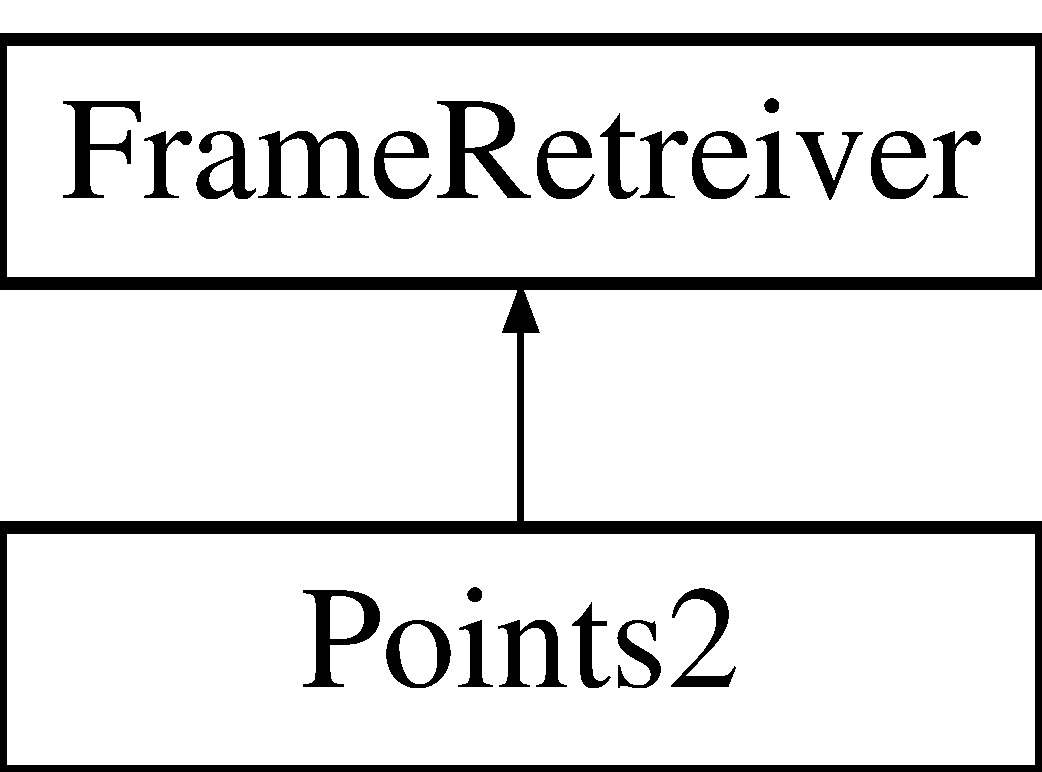
\includegraphics[height=2cm]{class_points2}
\end{center}
\end{figure}
\subsection*{Sygnały}
\begin{DoxyCompactItemize}
\item 
\hypertarget{class_points2_a40606e5bff8ad0c1fc1887669d6e8e6e}{
void {\bfseries bobjects} (BObList $\ast$list)}
\label{class_points2_a40606e5bff8ad0c1fc1887669d6e8e6e}

\end{DoxyCompactItemize}
\subsection*{Metody publiczne}
\begin{DoxyCompactItemize}
\item 
\hypertarget{class_points2_a8ae4636b6fcd263753884959bb7d9ede}{
{\bfseries Points2} (\hyperlink{class_video_input}{VideoInput} $\ast$input)}
\label{class_points2_a8ae4636b6fcd263753884959bb7d9ede}

\item 
\hypertarget{class_points2_af46dd0cd21f73b3214d5f766349b8450}{
void {\bfseries retreiveFrame} (cv::Mat \&)}
\label{class_points2_af46dd0cd21f73b3214d5f766349b8450}

\end{DoxyCompactItemize}
\subsection*{Statyczne metody publiczne}
\begin{DoxyCompactItemize}
\item 
\hypertarget{class_points2_af00905a8a3803e51af17d1d3dbd7f33c}{
static void {\bfseries addPoint} (int, int)}
\label{class_points2_af00905a8a3803e51af17d1d3dbd7f33c}

\end{DoxyCompactItemize}
\subsection*{Statyczne atrybuty publiczne}
\begin{DoxyCompactItemize}
\item 
\hypertarget{class_points2_a47f061a9802f8541f71ff3c805bd457f}{
static CvPoint {\bfseries pt} = cvPoint(0,0)}
\label{class_points2_a47f061a9802f8541f71ff3c805bd457f}

\item 
\hypertarget{class_points2_a27c9b3b569a0ac996490da0c6721408a}{
static int {\bfseries add\_\-remove\_\-pt} = 0}
\label{class_points2_a27c9b3b569a0ac996490da0c6721408a}

\end{DoxyCompactItemize}


Dokumentacja dla tej klasy została wygenerowana z plików:\begin{DoxyCompactItemize}
\item 
points.h\item 
moc\_\-points.cpp\item 
points.cpp\end{DoxyCompactItemize}

\hypertarget{class_video_input}{
\section{Dokumentacja klasy VideoInput}
\label{class_video_input}\index{VideoInput@{VideoInput}}
}
\subsection*{Sloty publiczne}
\begin{DoxyCompactItemize}
\item 
\hypertarget{class_video_input_a78e2d773100160be101d3c48ecdfb910}{
void {\bfseries safelyStop} ()}
\label{class_video_input_a78e2d773100160be101d3c48ecdfb910}

\end{DoxyCompactItemize}
\subsection*{Metody publiczne}
\begin{DoxyCompactItemize}
\item 
\hypertarget{class_video_input_a136409a2c510d131dd25b00796ebb9a6}{
{\bfseries VideoInput} (int frameRate)}
\label{class_video_input_a136409a2c510d131dd25b00796ebb9a6}

\item 
\hypertarget{class_video_input_ac2370a0c1ea0d4b1ce36c2f9678530a4}{
void {\bfseries addObserver} (\hyperlink{class_frame_retreiver}{FrameRetreiver} $\ast$)}
\label{class_video_input_ac2370a0c1ea0d4b1ce36c2f9678530a4}

\item 
\hypertarget{class_video_input_afc3bab19893d3e49284ab8b8101b9d1f}{
void {\bfseries delObserver} (\hyperlink{class_frame_retreiver}{FrameRetreiver} $\ast$)}
\label{class_video_input_afc3bab19893d3e49284ab8b8101b9d1f}

\item 
\hypertarget{class_video_input_a498cc39dce8940616e9d1811953bf920}{
void {\bfseries setFrameRate} (float frameRate)}
\label{class_video_input_a498cc39dce8940616e9d1811953bf920}

\item 
\hypertarget{class_video_input_aa172de34ebd4e1f1e7c63548fb406f39}{
float {\bfseries getFrameRate} ()}
\label{class_video_input_aa172de34ebd4e1f1e7c63548fb406f39}

\item 
\hypertarget{class_video_input_a95deb1fbd0ab027a4208b7432dedcdc9}{
unsigned long {\bfseries getSleepUTime} ()}
\label{class_video_input_a95deb1fbd0ab027a4208b7432dedcdc9}

\end{DoxyCompactItemize}
\subsection*{Metody chronione}
\begin{DoxyCompactItemize}
\item 
\hypertarget{class_video_input_a653a4568756629a94a3b6e2697973864}{
virtual void {\bfseries run} ()}
\label{class_video_input_a653a4568756629a94a3b6e2697973864}

\end{DoxyCompactItemize}


Dokumentacja dla tej klasy została wygenerowana z plików:\begin{DoxyCompactItemize}
\item 
videoinput.h\item 
videoinput.cpp\end{DoxyCompactItemize}

\printindex
\end{document}
